\section{Thermal-Hydraulics Analysis}
Preliminary checks were performed to validate the coolant properties, including density, viscosity, and thermal conductivity, at the coolant inlet temperature.

The heat transfer coefficient between the coolant and cladding was calculated using Nusselt number correlations, ensuring accurate representation of the thermal exchange process.

Figure~\ref{fig:thermal_hydraulics} presents the axial power profile. The computed heat transfer coefficient in the cold geometry was determined to be:
\[
\alpha_{\text{coolant}} = 139.98 \, \frac{\text{kW}}{\text{m}^2 \cdot \text{K}}
\]

\begin{figure}[H]
    \centering
    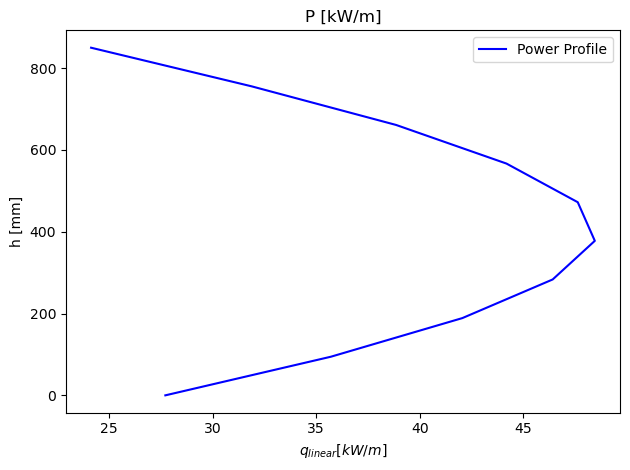
\includegraphics[width=0.6\textwidth]{power_profile.png}
    \caption{Axial power profile used in the thermal-hydraulics analysis.}
    \label{fig:thermal_hydraulics}
\end{figure}
